\documentclass[fleqn,reqno,10pt]{article}

\usepackage{myarticlestyledefault}

\usepackage{pgfplots}

\begin{document}

ae ntr

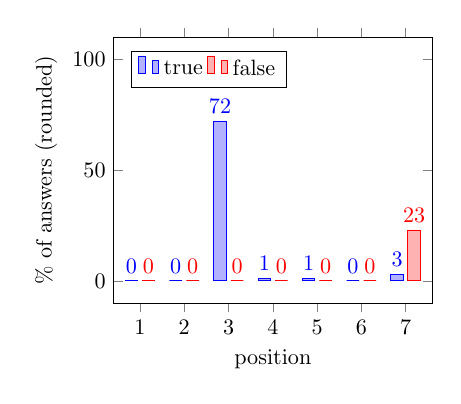
\begin{tikzpicture}[scale=0.8]

      \begin{axis}[ybar, 
                  enlarge x limits=0.1,
                  enlarge y limits=0.1,
                  legend style={at={(0.3,0.95)}, anchor=north, legend columns=-1},
                  ylabel={\% of answers (rounded)}, 
                  xlabel={position}, 
                  symbolic x coords={1, 2, 3, 4, 5, 6, 7}, 
                  xtick=data, 
                  nodes near coords,
                  nodes near coords align={vertical}, 
                  x=20, y=1,
                  ymin = 0, ymax = 100,
                  bar width=2mm
        ]

        \addplot coordinates {(1,0) (2,0) (3,72) (4,1) (5,1) (6,0) (7,3)};

        \addplot coordinates {(1,0) (2,0) (3,0) (4,0) (5,0) (6,0) (7,23)};

        \legend{true, false}

      \end{axis}

    \end{tikzpicture}

ae akz



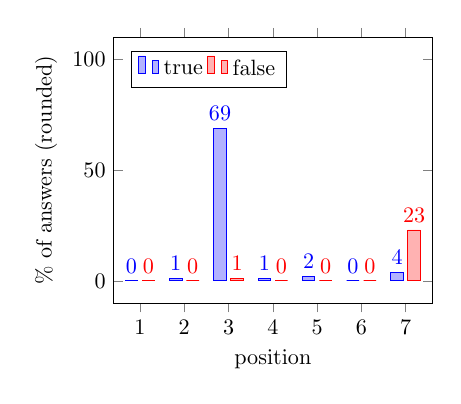
\begin{tikzpicture}[scale=0.8]

      \begin{axis}[ybar, 
                  enlarge x limits=0.1,
                  enlarge y limits=0.1,
                  legend style={at={(0.3,0.95)}, anchor=north, legend columns=-1},
                  ylabel={\% of answers (rounded)}, 
                  xlabel={position}, 
                  symbolic x coords={1, 2, 3, 4, 5, 6, 7}, 
                  xtick=data, 
                  nodes near coords,
                  nodes near coords align={vertical}, 
                  x=20, y=1,
                  ymin = 0, ymax = 100,
                  bar width=2mm
        ]

        \addplot coordinates {(1,0) (2,1) (3,69) (4,1) (5,2) (6,0) (7,4)};

        \addplot coordinates {(1,0) (2,0) (3,1) (4,0) (5,0) (6,0) (7,23)};

        \legend{true, false}

      \end{axis}

\end{tikzpicture}

ge ntr

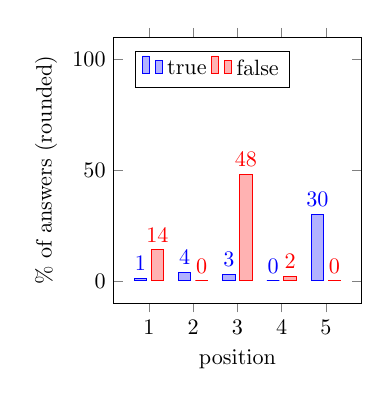
\begin{tikzpicture}[scale=0.8]

      \begin{axis}[ybar, 
                  enlarge x limits=0.2,
                  enlarge y limits=0.1,
                  legend style={at={(0.4,0.95)}, anchor=north, legend columns=-1},
                  ylabel={\% of answers (rounded)}, 
                  xlabel={position}, 
                  symbolic x coords={1, 2, 3, 4, 5}, 
                  xtick=data, 
                  nodes near coords,
                  nodes near coords align={vertical}, 
                  x=20, y=1,
                  ymin = 0, ymax = 100,
                  bar width=2mm
        ]

        \addplot coordinates {(1,1) (2,4) (3,3) (4,0) (5,30)};

        \addplot coordinates {(1,14) (2,0) (3,48) (4,2) (5,0)};

        \legend{true, false}

      \end{axis}

\end{tikzpicture}

ge akz

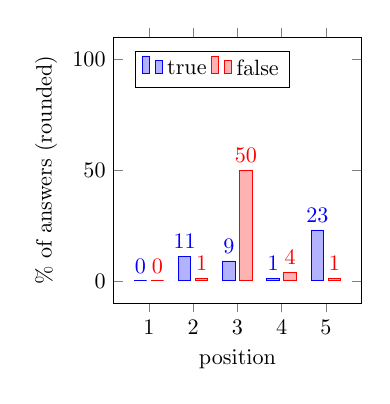
\begin{tikzpicture}[scale=0.8]

      \begin{axis}[ybar, 
                  enlarge x limits=0.2,
                  enlarge y limits=0.1,
                  legend style={at={(0.4,0.95)}, anchor=north, legend columns=-1},
                  ylabel={\% of answers (rounded)}, 
                  xlabel={position}, 
                  symbolic x coords={1, 2, 3, 4, 5}, 
                  xtick=data, 
                  nodes near coords,
                  nodes near coords align={vertical}, 
                  x=20, y=1,
                  ymin = 0, ymax = 100,
                  bar width=2mm
        ]

        \addplot coordinates {(1,0) (2,11) (3,9) (4,1) (5,23)};

        \addplot coordinates {(1,0) (2,1) (3,50) (4,4) (5,1)};

        \legend{true, false}

      \end{axis}

\end{tikzpicture}


\printbibliography[heading=bibintoc]

\end{document}
